\chapter{Domain Model}

\vspace{-5pt}
%kommentar
\begin{figure}[H]
	\centering
	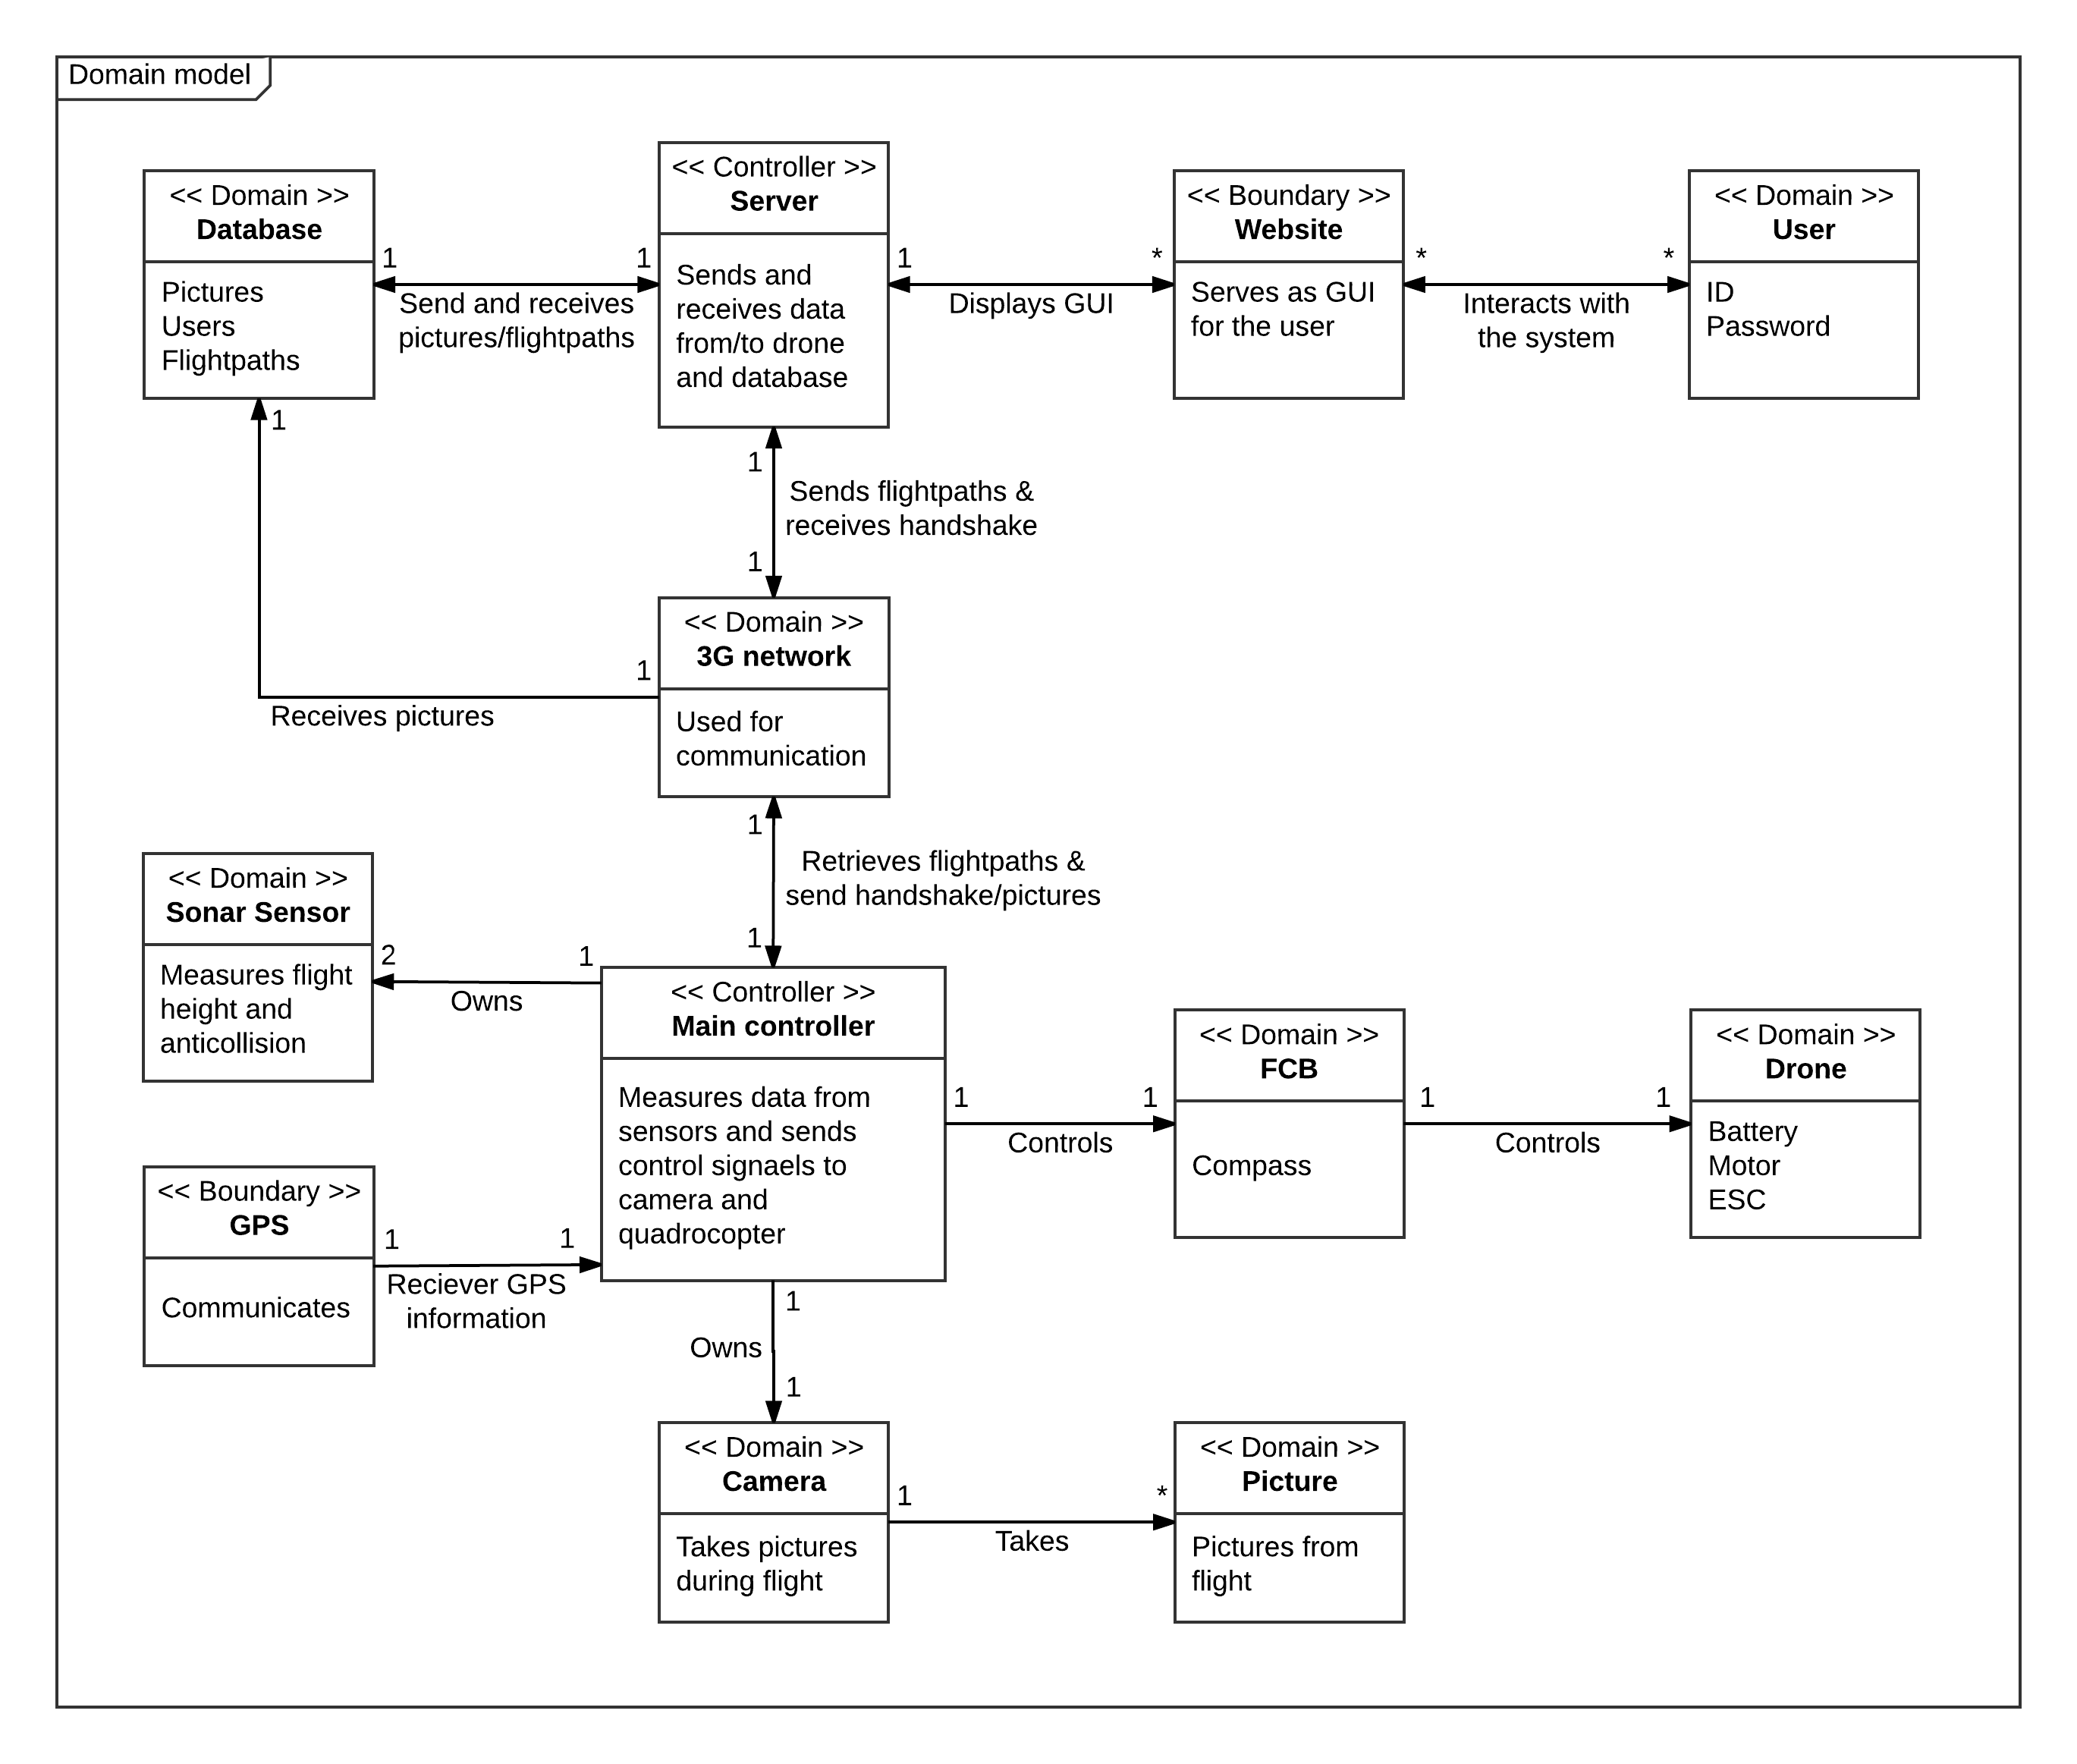
\includegraphics[width=1.1\textwidth]{Billeder/domain_model.png}
	\vspace{-5pt}
	\caption{Domain model}
	\label{fig:domain_model}
\end{figure}

På domain modellen ses det overordnet design af systemet. På figuren tydelige gøres det at al kommunikation imellem server og arduino køre over 3G netværket. Når arduinoen tændes sender arduinoen et handshake signal til serveren for at fortælle at den er online. Efter følgende pinger arduinoen serveren hvert 30 sekund for at fortælle serveren at den er online. Når serveren modtager handshake fra arduinoen vil dette blive markeret på websitet. Useren har mulighed for at gemme fly ruter i databasen til senere brug. Billeder taget under flyvning som har fået accept af useren, vil blive gemt i databasen.